\section{Results} \label{sec:results}

\subsection{Determine the interaction J}
We have tried to determine the value of J using both linear regression (OLS, Ridge and Lasso) and neural networks. In project 1, we found our implementation of OLS, Ridge and Lasso to give the same result as Scikit Learn, and we will in this project stick to Scikit Learn due to its quickness. [Ref. project 1]
\begin{table} [H]
	\caption{Mean Square Error and R$^2$-score of the obtained J obtained from linear regression and neural network.  , where noise was added to the data. The parameters used were $\lambda=1e-5$ (penalty), $\eta=1e-4$ (learning rate), $\text{niter}=1e5$ (number of iterations) and $\mathcal{N}(0, \sigma^2=0.1)$ (noise). See text for more information.}
	\begin{tabularx}{\textwidth}{l|XXX|XX} \hline\hline
		\label{tab:franke_error}
		& \multicolumn{3}{c}{\textbf{Linear regression}}&\multicolumn{2}{c}{\textbf{Neural networks}}\\ \hline
		&OLS&Ridge&Lasso&OLS&CE\\ \hline
		MSE & 0.008494 & 0.009119 & 0.008494 & 0.9048 & 0.8956 \\
		R2 & 0.009128 & 0.009651 & 0.009128 & 0.8977 & 0.8895 \\ \hline
	\end{tabularx}
\end{table}

\subsubsection{Linear regression}
\subsubsection{Neural networks}

\subsection{Classifying the phase}
\subsubsection{Logistic regression}
\subsubsection{Neural networks}



\iffalse
\begin{figure} [H]%
	\centering
	\subfloat[Lambda vs. R2-score]{{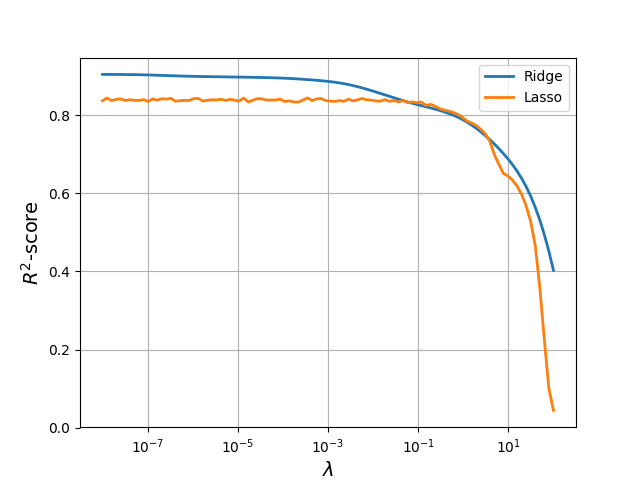
\includegraphics[width=7cm]{../plots/lambda_R2score.png} }}%
	\subfloat[Variance vs. R2-score]{{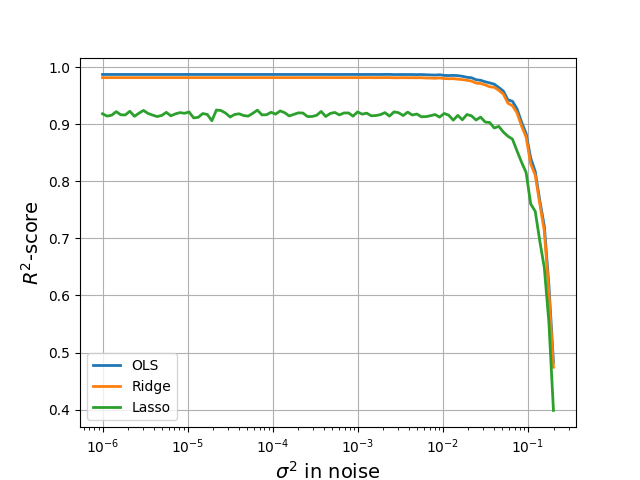
\includegraphics[width=7cm]{../plots/var_R2score.png} }}
	\caption{R$^2$-score plotted as a function of the penalty $\lambda$ (a) and as a function of the noise (b). $\lambda\in[10^{-8},10^2]$ in (a) and $\sigma^2\in[10^{-6},10^{-0.7}]$ in (b). The other parameters used were $\lambda=1e-5$ (penalty, was held constant for (b) only), $\eta=1e-4$ (learning rate), $niter=1e5$ (number of iterations) and $\mathcal{N}(0, \sigma^2=0.1)$ (noise, was held constant for (a) only).}%
	\label{fig:R2_scores}
\end{figure}
\fi 


